\documentclass[10pt]{beamer}
\setbeamertemplate{navigation symbols}{\insertlogo}

%\documentclass[handout,dvips,11pt,grey]{beamer}

%\usetheme{Goettingen}
%\usetheme{Warsaw}
\usetheme{Hannover}

%\usepackage{tikz,pgf}
\usepackage{xcolor}
\usepackage{multicol}
\usepackage{amsmath,amsthm,amssymb}
%\usepackage{epstopdf}
\usepackage{xspace}
\usepackage{wrapfig}

\usepackage{verbatim}
%\usepackage{circuitikz}
%\usepackage{graphicx}
\usepackage{comment}
%\usepackage{array}
\usepackage{coffee4}

\usepackage{fontawesome}


\title{Matchmaking for Industry}
\subtitle{Estimating Expertise from Issue Tickets with Topic Modeling}
\author{Philip Robinson}
\date{\today}
\institute{Presented to PyData PDX \\ Work from NASA - Jet Propulsion Lab}

\DeclareMathOperator*{\argsort}{argsort}

\logo{
\includegraphics[height=.7cm]{./pdx.png}}

\begin{document}

\begin{frame}
  \titlepage

\end{frame}


\begin{frame}{Presentation Overview}
  \tableofcontents

\end{frame}

\section{Introduction}

\begin{frame}{Philip Robinson}

  That's me!

  \vspace{1em}

  \begin{multicols}{2}
    \begin{figure}
    
\includegraphics[width=\columnwidth]{./philip.jpg}
    \caption{JunGlow Love, 2015 PDX}
    \end{figure}

    \begin{itemize}
    \item[\faTwitter] \texttt{@timedebtor}
    \item[\faGithub] \texttt{@probinso}
    \item[\faEnvelope] probinso@protonmail.com
    \item Work at GrammaTech
    \item Alumni at OHSU \& WWU
    \end{itemize}
  \end{multicols}

\end{frame}

\section{Problem}

\begin{frame}{Problem Description}
  
\includegraphics[width=0.4\textwidth]{./logo.png}
  \begin{quote}
    {\footnotesize
    NASA's Jet Propulsion Lab uses a custom ticketing system to
    assign experts to ``mission critical late stage anomalies''.
    The ticketing system is used to document progress, contributors, and
    solutions against these tickets.
    A ticket manager is responsible for assigning the first contributors \&
    experts to solve a ticket.
    }
  \end{quote}

  \begin{itemize}
  \item Recruiting impactful teams is very time expensive
  \item Incomplete understanding of candidate expertise or ticket topic
  \item Uneven distribution of assignment
  \item Find experts from other divisions and projects
  \end{itemize}

\end{frame}

\begin{frame}{What is our generalized goal?}

  \begin{quote}
    We have a ticketing system used to track progress in solving specialized tasks.
  \end{quote}

  \begin{enumerate}
  \item A first response needs to build a candidate solution team
  \item We have a textual description of solved tasks with attribution
  \item We would like to automatically identify candidates
  \end{enumerate}


  \begin{quote}
    Can we estimate expertise of candidates given a ticket?
  \end{quote}
\end{frame}

\begin{frame}{Proposal - Author Modeling}
  {\bf Model Expertise of SME by tickets and attributions}

  \begin{quote}
    Author modeling
    has been used to measure attribution\cite{Rexha2018} and
  contribution\cite{AldebeiHJ016}. Author-Topic Modeling (ATM) establishes a strategy to
  map both authors and documents to the same topic-space over a vocabulary\cite{Rosen-Zvi2004}.
  \end{quote}

  \begin{center}
    If I am the author, then I should be an expert on the contents
  \end{center}
\end{frame}

\section{Topic Modeling}

\begin{frame}{What is Topic Modeling}
  {\bf I love LDA based topic modeling}

  \begin{quote}
    Topic modeling\cite{Ren2013} is a text processing technique for learning topics from a collection of documents. This is usually used as a strategy to describe documents in a comparable low dimensional space or an exploratory tool for grouping document collections.
  \end{quote}
\end{frame}

\newcommand{\Food}[1]{\colorbox{orange!30}{#1}\xspace}
\newcommand{\Travel}[1]{\colorbox{blue!30}{#1}\xspace}
\newcommand{\Time}[1]{\colorbox{green!30}{#1}\xspace}
\newcommand{\Document}[1]{\fbox{\begin{minipage}{\columnwidth}#1\end{minipage}}}

\begin{frame}{Examples}
{\bf In practice, this requires many more documents}

  \begin{multicols}{2}

    \Document{
      The \Travel{Tourist} huddles in the \\ \Travel{station} While slowly \Time{night} gives way to \Time{dawn}; He finds a certain fascination In knowing all the \Travel{trains} are gone.
    }

    \vspace{.25em}

    \Document{
      The Governess up in the attic \\Attempts to make a cup of \Food{tea}; Her mind grows \Time{daily} more erratic From cold and \Food{hunger} and ennui.
    }

    \vspace{.25em}

    \Document{
      The Journalist surveys the slaughter, The best in \Time{years} without a doubt; He pours himself a \Food{gin} and \Food{water} and wonders how it came about.
    }

    \columnbreak

    \begin{itemize}
    \item \Food{Food}
    \item \Travel{Travel}
    \item \Time{Time}
    \end{itemize}

    \vspace{1em}

    From this annotation we know that Document 2 and 3 are about \Food{Food} and \Time{Time}
  \end{multicols}

\end{frame}

\begin{frame}{What can I do with topic models?}
  \begin{itemize}
  \item Cluster documents by topic
  \item Define interpretable topics that describe a corpus
  \item Dimmentionality reduction of documents
  \item Corpus aware document similarities
  \end{itemize}

  \begin{quote}
    Topic modeling can usually be extended to address many other problems, and document embedding can be used to inform downstream models.
  \end{quote}
\end{frame}

\begin{comment}
\begin{frame}{Applications of Topic Modeling}

  \begin{multicols}{4}

  \begin{figure}
  \includegraphics[width=\columnwidth]{full2.png}

  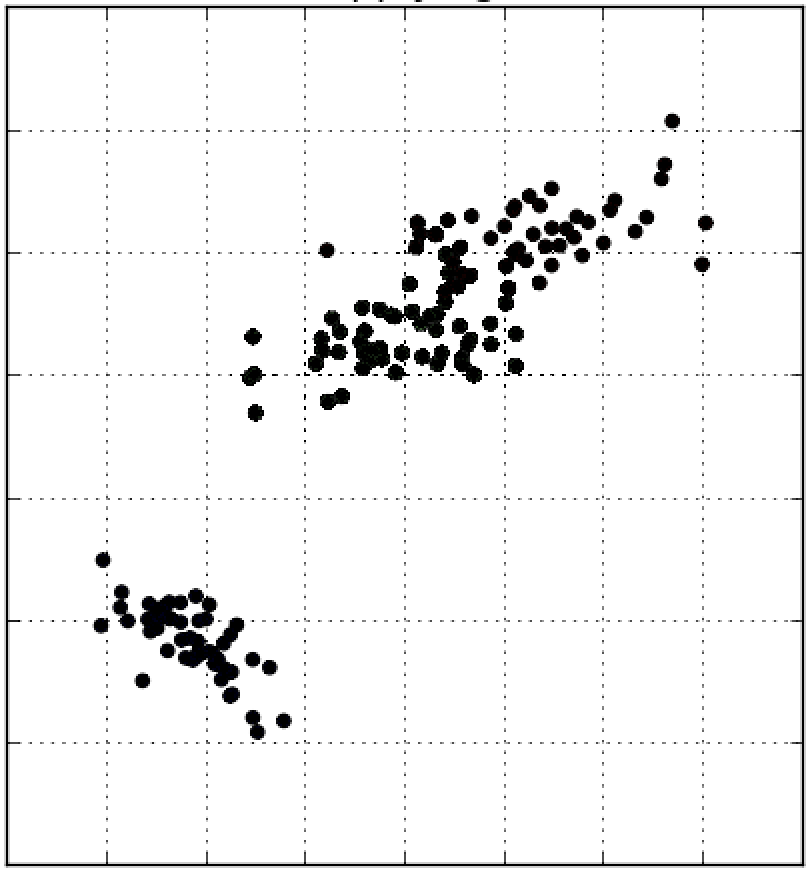
\includegraphics[width=.8\columnwidth]{reduced.png}
  \caption{Dimmentionality Reduction}
  \end{figure}
  \columnbreak

  \hfill
    \begin{figure}
  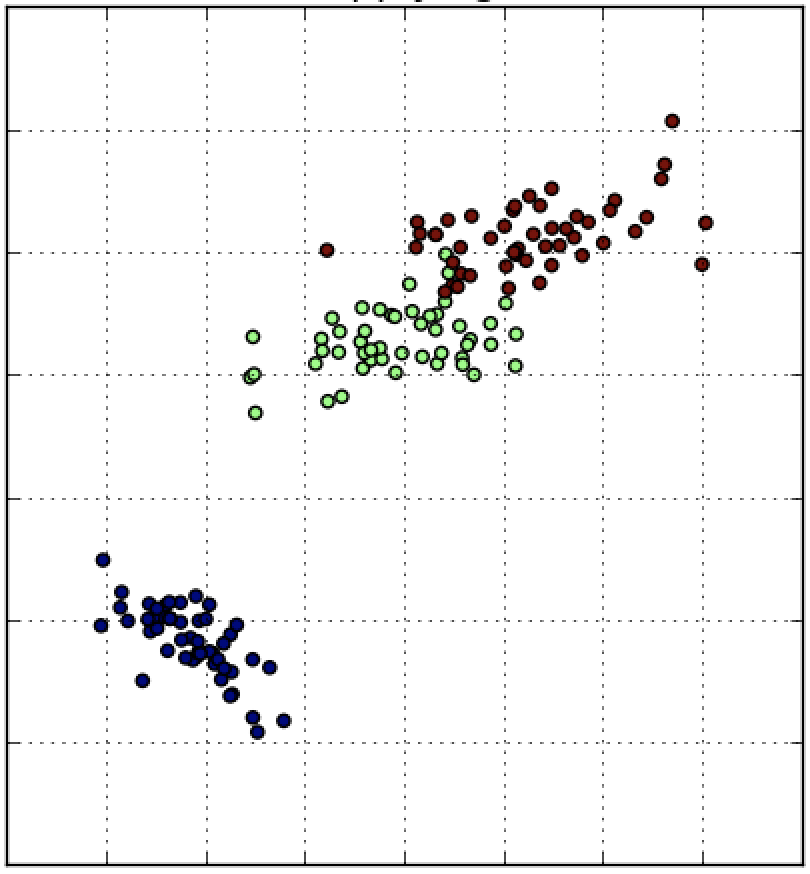
\includegraphics[width=\columnwidth]{cluster.png}
  \caption{Cluster Points}
  \end{figure}
    \columnbreak

  \hfill
    \begin{figure}
  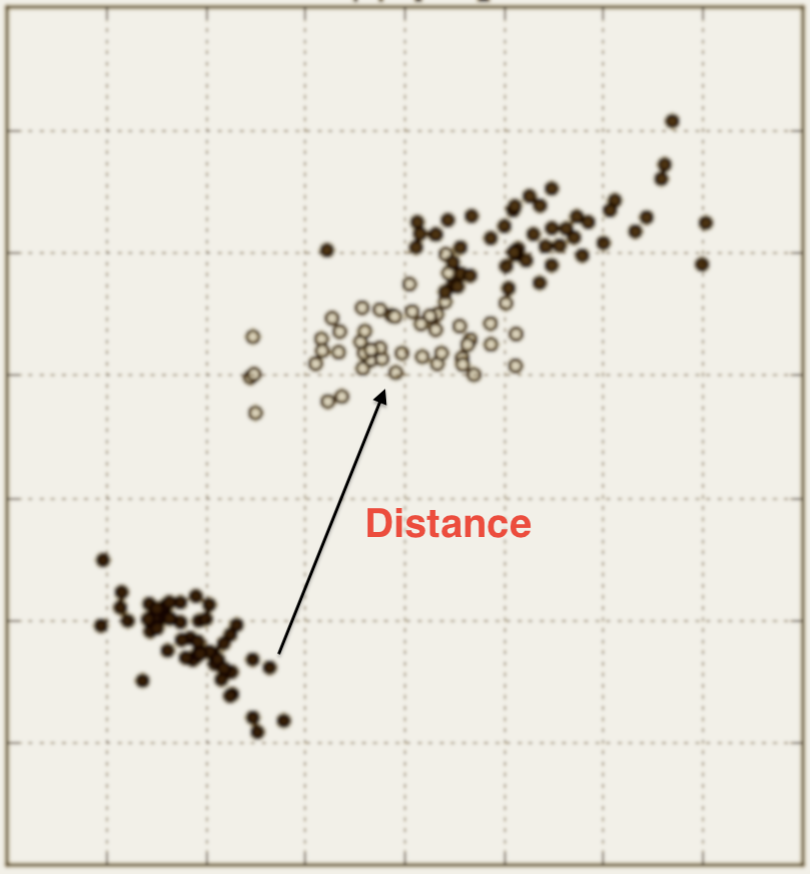
\includegraphics[width=\columnwidth]{dist.png}
  \caption{Exploratory Data Analysis}
  \end{figure}
    \columnbreak

  \hfill
    \begin{figure}
  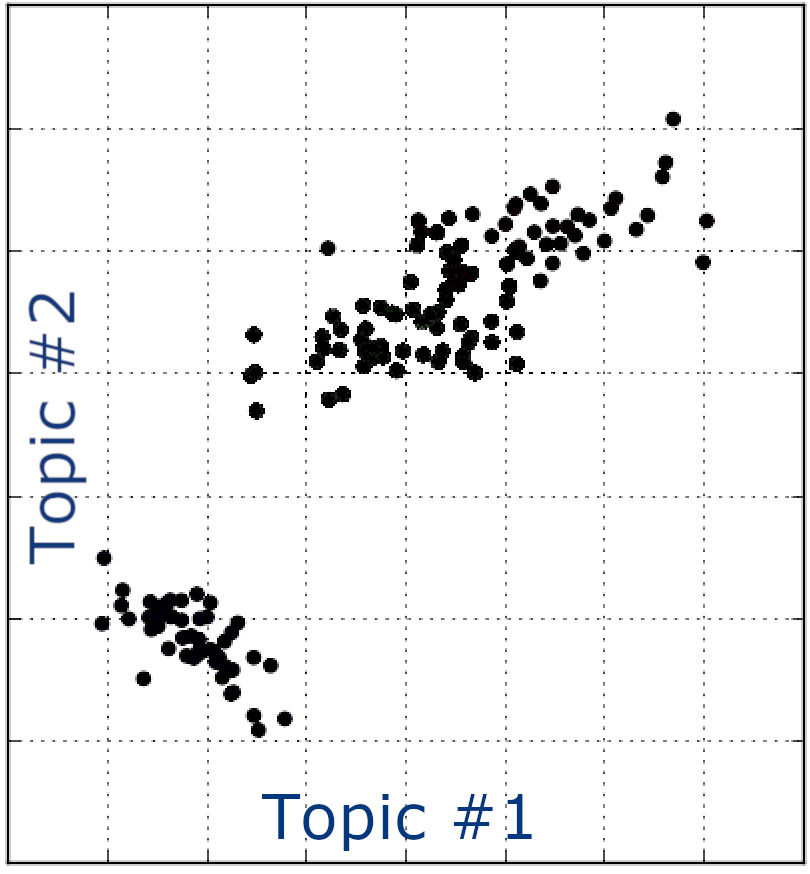
\includegraphics[width=\columnwidth]{topicanalysis.png}

  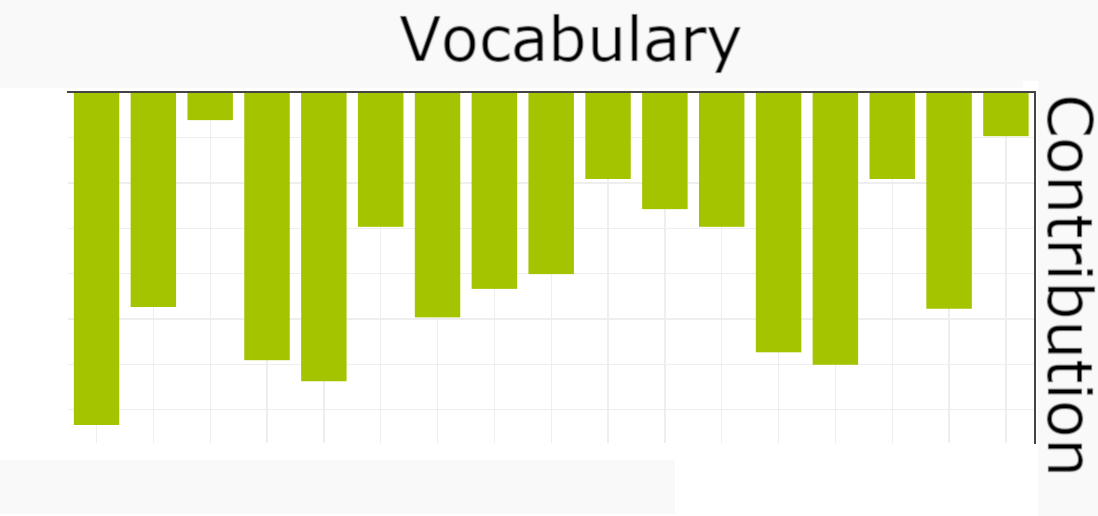
\includegraphics[width=\columnwidth]{bar-simple.png}
  \caption{Analysis of Topics}
  \end{figure}

  \end{multicols}

\end{frame}
\end{comment}

\section{Latent Dirichlet Allocation}

\begin{frame}{Latent Dirichlet Allocation\cite{BleiNg2010}}
  {\bf Bayesian extension to PLSA\cite{DBLP:journals/corr/abs-1301-6705} extends LSA/SVD\cite{deerwester-indexing-1990}}

  \begin{multicols}{2}

  \begin{itemize}
  \item Represent document as Bag-of-Words\footnote{equivalent to multinomial over the vocabulary}
  \item Model/Fit topics as mixture of words
  \item Documents are projected into or sampled from topic-space-distribution
  \end{itemize}

  \begin{figure}
  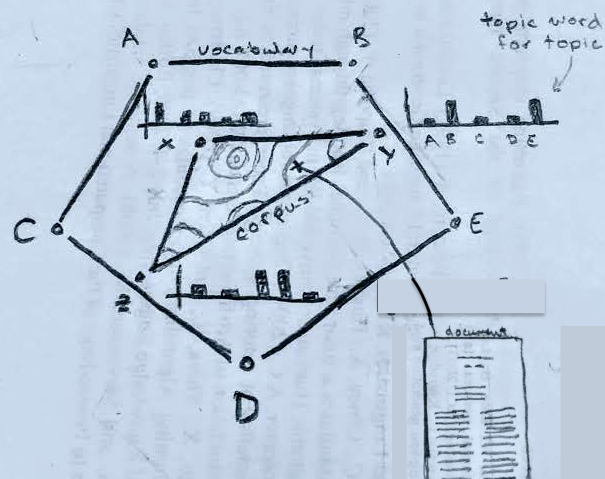
\includegraphics[width=\columnwidth]{./lda-draw.png}
  \caption{Latent Dirichlet Allocation}
  \end{figure}

  \end{multicols}

\end{frame}


\begin{frame}{Looking at top words}
  {\bf Mitigating apophenia is hard, topics difficult to interpret}

  \begin{multicols}{3}
    Topic \#1
    \begin{itemize}
    \item server
    \item connected
    \item access
    \item workstation
    \item outage
    \item user
    %\item service
    %\item restart
    \end{itemize}

    \columnbreak

    Topic \#2
    \begin{itemize}
    \item mode
    \item instrument
    \item safe
    \item spacecraft
    \item anomaly
    \item recovery
    %\item event
    %\item control
    \end{itemize}

    \columnbreak

    Topic \#3
    \begin{itemize}
    \item uplink
    \item station
    \item dsn
    %\item spacecraft
    \item lock
    \item ace
    %\item bps
    \item radiation
    \end{itemize}

  \end{multicols}

  \begin{quote}
    Although the model better describes our generation process, from the perspective of topics, it can be difficult to know what these topics actually represent.
  \end{quote}
\end{frame}


\begin{frame}{Extensions}
  \begin{quote}
    Extensability is what makes LDA most interesting
  \end{quote}

  \begin{itemize}
  \item[$\rightarrow$] Author Topic Model\cite{Rosen-Zvi2004}
  \item Correlated Topic Model\cite{NIPS2005_2906}
  \item Biterm Topic Model\cite{Yan2013,Chen2015}
  \item Twitter Topic Model\cite{LimCB16}
  \item Supervised LDA\cite{NIPS2007_3328}
  \item Hierarchical Dirichlet Process\cite{Teh:EtAl:06}
  \end{itemize}
\end{frame}

\section{Application}

\begin{frame}{Approach}
  {\bf Author-Topic-Modeling}

% Fitting authorship as a generative model allows us to mathematically abstract and describe a provided corpus, allowing us to ask deeper questions about incoming documents. We elect using the Author-Topic-Model (ATM) to ask the `most likely author' of a document, as a proxy for expertise.

  \begin{multicols}{2}

  \begin{itemize}
  \item Interpret doc as Bag-of-Words\footnote{equivalent to multinomial over vocabulary}
  \item Model/Fit topics as mixture of words
  \item Author \& document are projected into topic-space
  \item Measure distance from author to document
  \end{itemize}

  \begin{figure}
  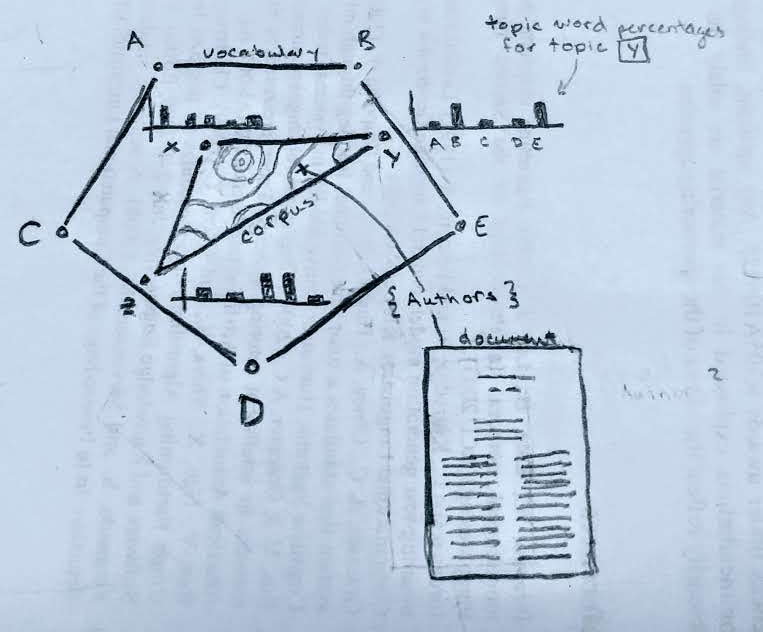
\includegraphics[width=\columnwidth]{./lda-draw.jpg}
  \caption{Latent Dirichlet Allocation}
  \end{figure}

  \end{multicols}

  \vspace{-2em}
  \begin{align*}
    T(x) &= \texttt{Project $x$ into topic-space} \\
    R_d &= \argsort_{a\in A} \left\{Distance(T(a),T(d))\right\}
  \end{align*}

\end{frame}


\section{Results}

\begin{frame}{Ranking}
  {\bf Seems to work}

  Given Authors/Experts in a ``Topic Space'' and a mapping from document to ``Topic Space'', we can rank experts for a document. %Ideally this is done with the probability of an author given a document, but presently we use distribution similarity metrics to rank authors.


  \begin{multicols}{2}
    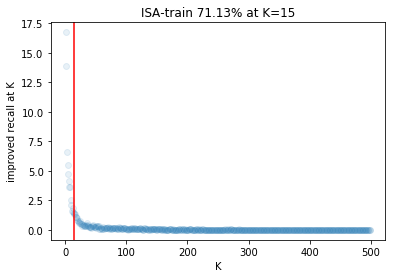
\includegraphics[width=\columnwidth]{./recall-train-isa.png}

    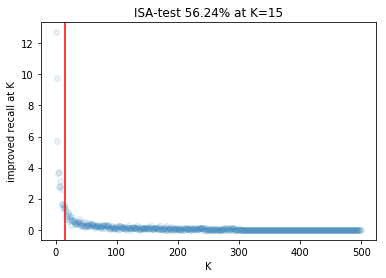
\includegraphics[width=\columnwidth]{./recall-test-isa.png}
  \end{multicols}

  K is cutoff for suggested candidates
\end{frame}

\begin{frame}{Receiving Candidates}
  {\bf Results begin at 4 words}

  It is possible to get interesting results at a document length of 4 words,
  however it is hard to know why these results are interesting.
  This is an example of directly searching for experts.

  \begin{multicols}{2}
    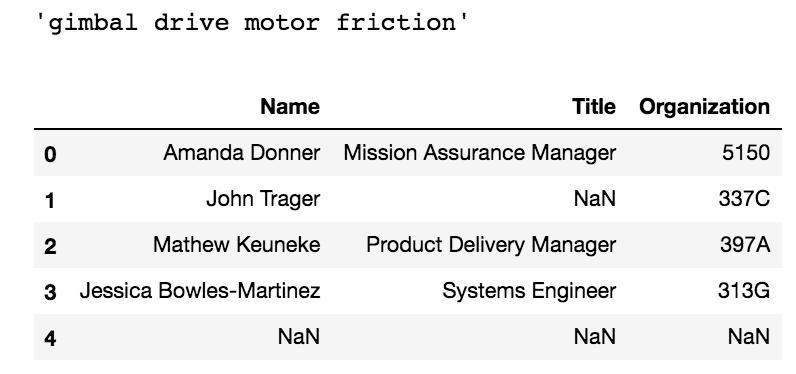
\includegraphics[width=\columnwidth]{query1.png}

    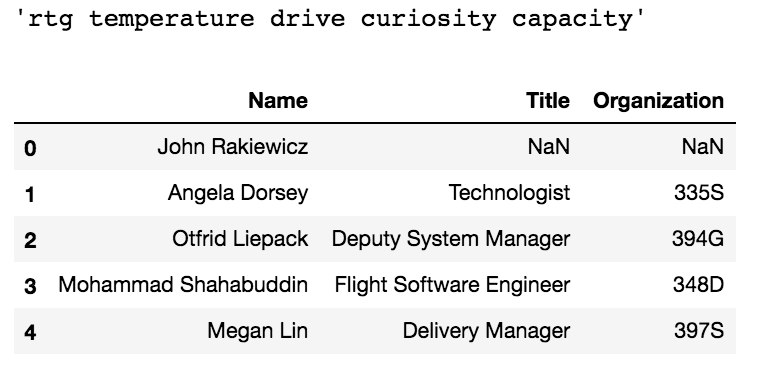
\includegraphics[width=\columnwidth]{query2.png}
  \end{multicols}

%  Documents queries generate better results. These examples are
%  currently unable to demo.

\end{frame}


\begin{frame}{How does word count effect recall?}
  {\bf Best results at 30 words}

  We are interested in understanding how much text is required to inform
  our model prediction. For these plots, we randomly subset texts for
  known ticket-expert pairs and observe the expert's new ranking.

  \begin{multicols}{2}
    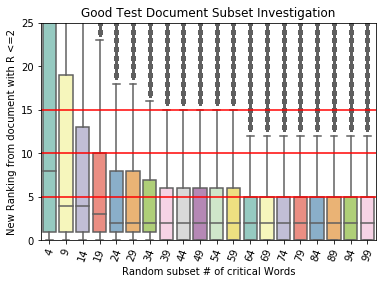
\includegraphics[width=\columnwidth]{low-ranked-downsample.png}
    Expert found in top 2\\
    24 critical words


    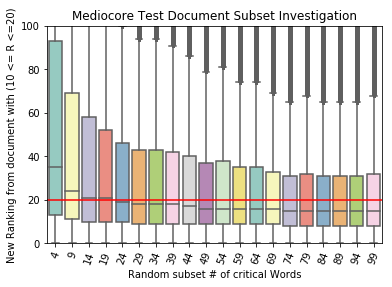
\includegraphics[width=\columnwidth]{mid-ranked-downsample.png}
    expert found in 10-20 range\\
    29 critical words
  \end{multicols}
\end{frame}

\section{Distances}

\begin{frame}{Distance Measures}
  {\bf Testing distances is cheaper than understanding them}

  \begin{quote}
    Hellinger distance\cite{krstovski2013efficient} commonly used for distance of points in Probability Simplex. The domain of the Dirichlet distribution can be thought of as a simplex over multinomial distributions.\footnote{Most online examples use cosine distance, \\without justification}
  \end{quote}
\end{frame}


\begin{comment}
  \begin{frame}{Using this in Python\footnote{example in \texttt{scikit-learn}, I used \texttt{gensim}}}
  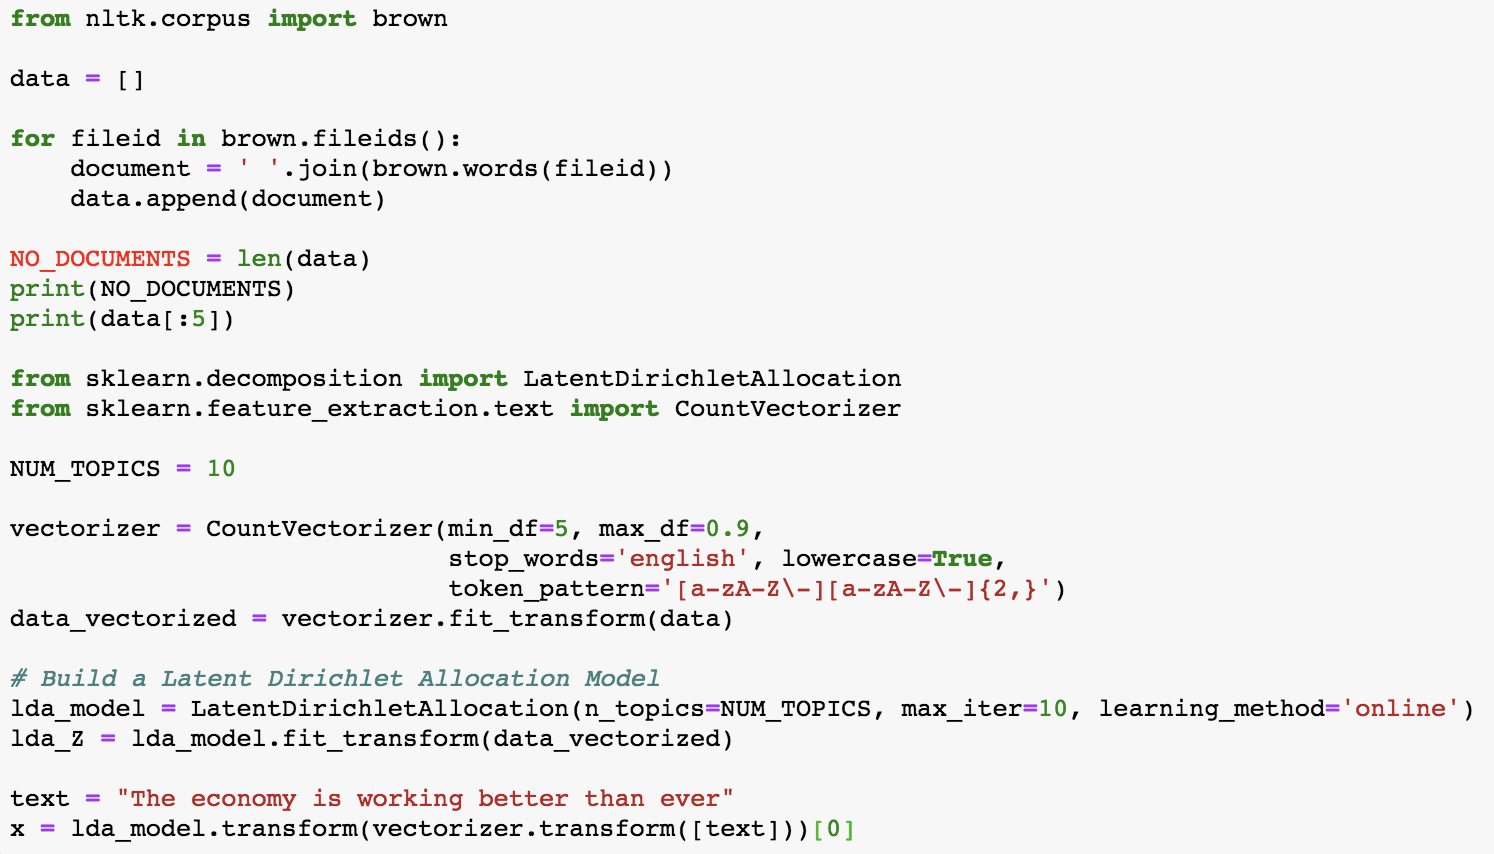
\includegraphics[width=\textwidth]{./implement.png}
\end{frame}
\end{comment}

\section{Evaluation}

\begin{frame}{Evaluation}
  {\bf Does our fit Dirichlet distribution describe our data or our understanding?}

  \begin{itemize}
  \item perplexity
  \item predictive power (Recall / Precision)
  \item coherence\cite{Roder2015,TACL582}
  \item visualization\cite{sievert-shirley-2014-ldavis,2012-termite}
  \item topic stability\cite{Yang2016}
  \item topic significance\cite{alsumait2009topic}
  \end{itemize}
\end{frame}

\begin{frame}{Perplexity}
  {\bf perplexity for prediction}

  \begin{quote}
    Perplexity is a measure of how poorly the model describes the data. Low perplexity indicates the distribution is a good description of the sample. For LDA this prioritizes dimensional reduction.
  \end{quote}

  \begin{align*}
    Perplexity(q) &= b^{-\frac{1}{N}\sum_{x \in X} log_b q(x)}
  \end{align*}

\end{frame}
\begin{frame}{Coherence}
  {\bf coherence for scorable EDA\footnote{exploratory data analysis}}
  \begin{quote}
    Topic coherence measures take the set of $N$ top words from a topic and sums a \texttt{confirmation measure}\footnote{like pointwize mutual information (PMI)} over the word pairs. Probabilities are estimated from sliding window over train and test corpora.
  \end{quote}

  \begin{align*}
    C_{Irvine} &= \frac{2}{N\cdot N-1}\sum_{i=1}^{N-1}\sum_{j=i+1}^N PMI(w_i, w_j)\\
    PMI(w_i, w_j) &= log(\frac{P(w_i, w_j)}{P(w_i)\cdot P(w_j)})
  \end{align*}
\end{frame}

\begin{frame}{Visualization (pyLDAvis)}
  {\bf Interpretable EDA}

    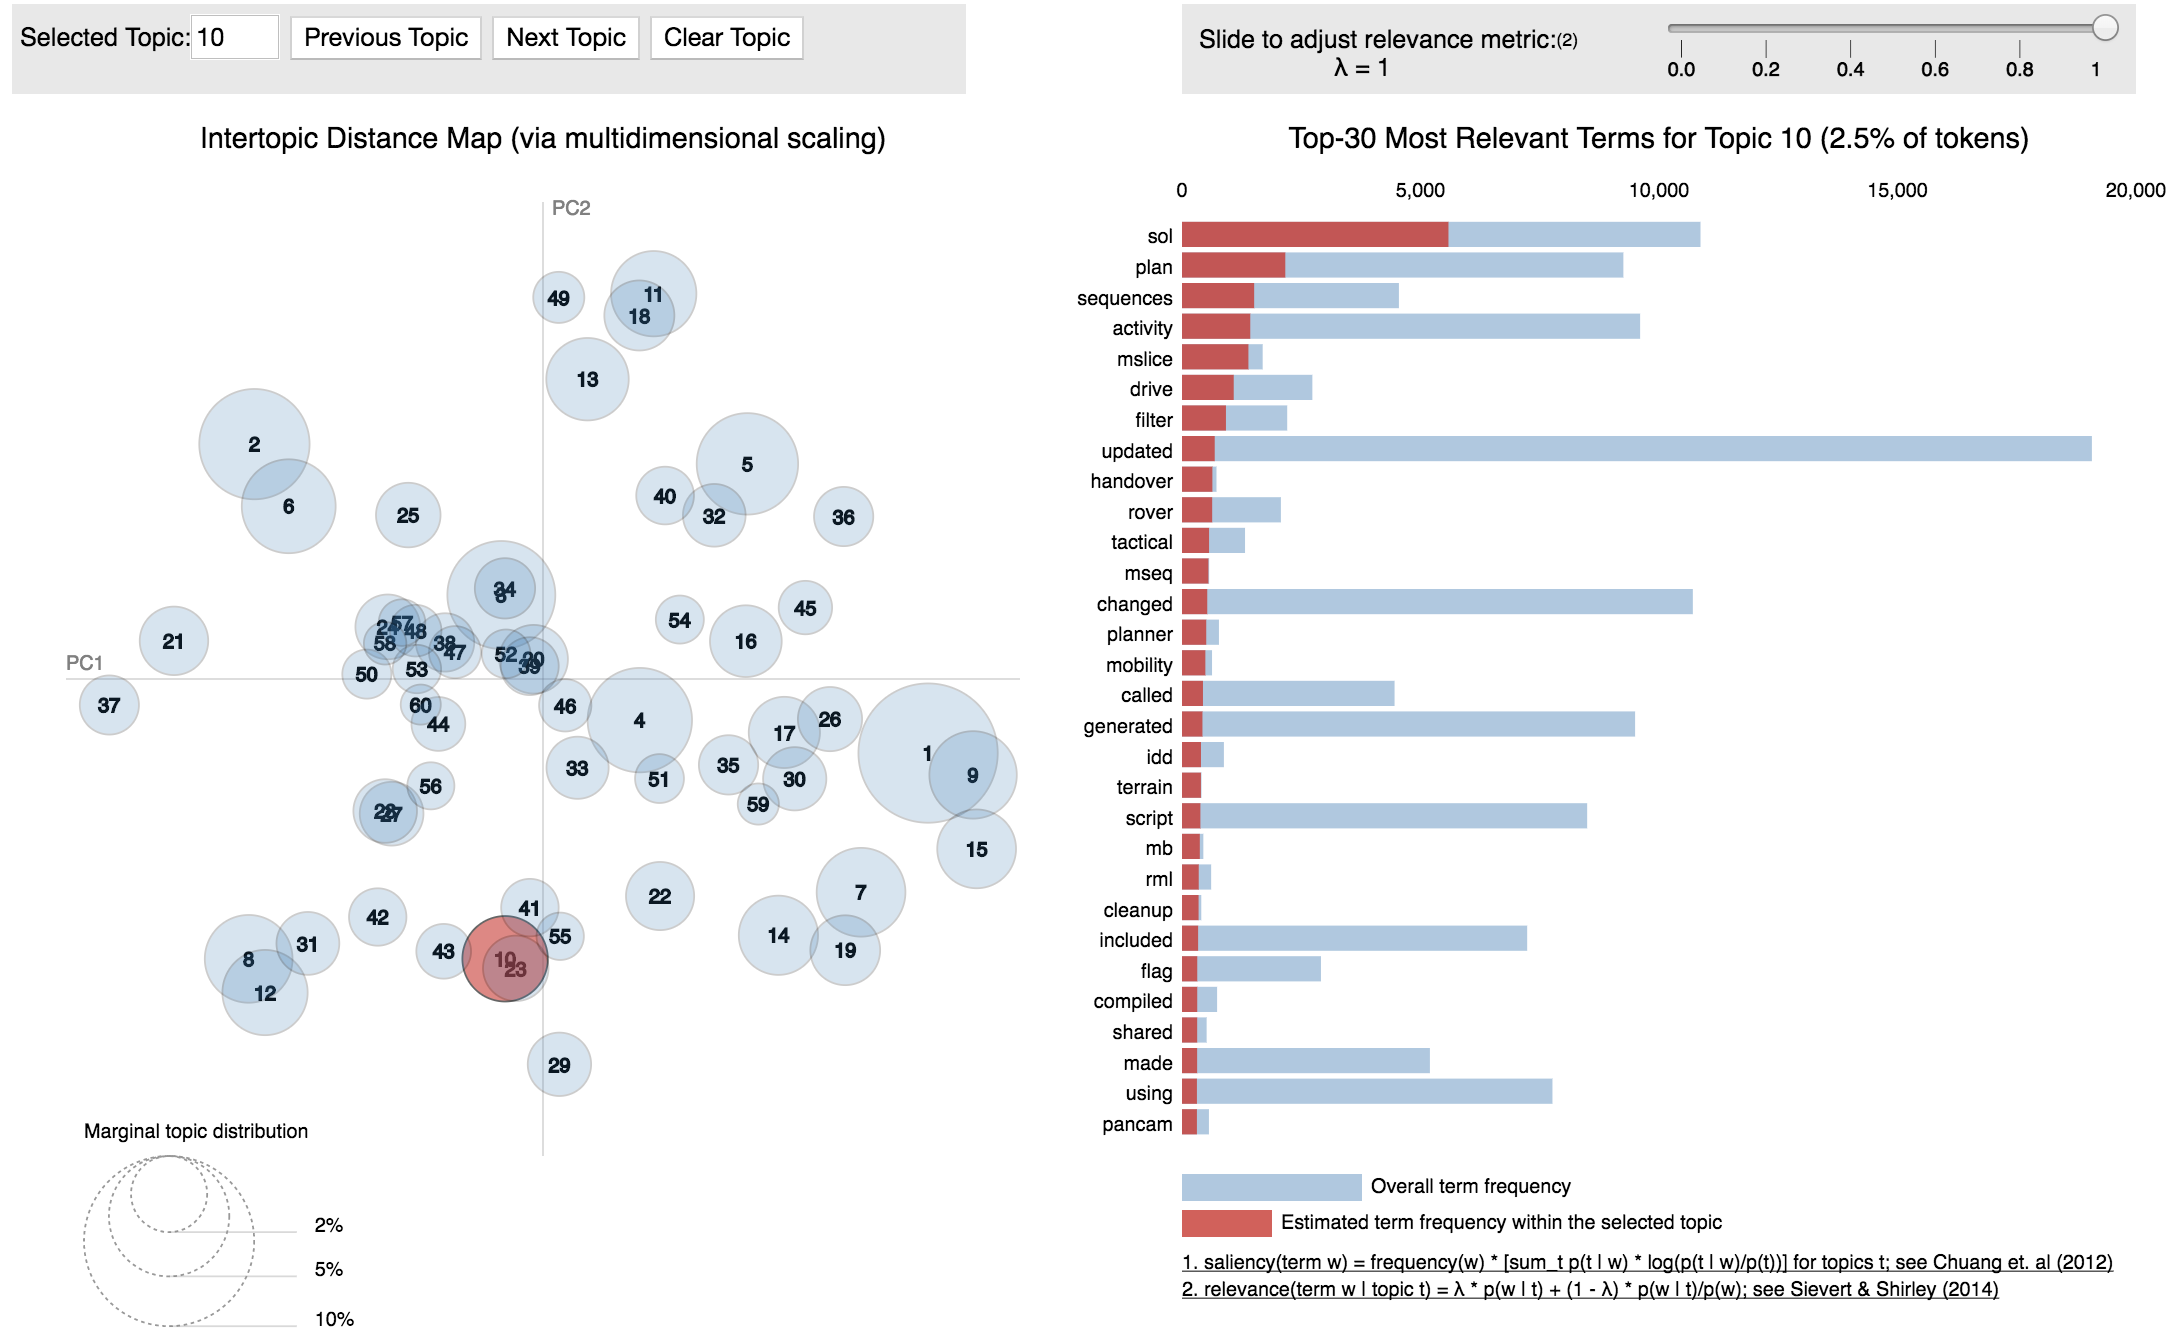
\includegraphics[width=\textwidth]{LDAvis.png}

\end{frame}


\begin{comment}
  \begin{frame}{Predictive Power}
  {\bf Depends on your downstream applications}

  \begin{quote}
    Does your client end up benefiting from the tool. This could be many measures like recall or click-through.
  \end{quote}
  \end{frame}
\end{comment}

\begin{frame}{Conclusion \& Questions}

\end{frame}

\section{Bibliography}

\begin{frame}[allowframebreaks]{Bibiography}
  \tiny
  \bibliography{references.bib}{}
\bibliographystyle{plain}

\end{frame}

\section{Cleaning and Preprocessing}

\begin{frame}{Text Pre-Processing}
{\bf Cleaning applies to most 'simple' NLP problems}

\begin{quote}
  Text normalization is custom to your corpus. Many of the steps are the same, but their application changes with the type of documents.
\end{quote}

  \begin{itemize}
  \item Normalize text
    \begin{itemize}
    \item Lowercase text
    \item[$\star$] Remove non-informative text patterns
    \end{itemize}
  \item Tokenization \& (Stemming | Lemmatization)
    \begin{itemize}
    \item[$\star$] pick a stemmer
    \item Stem \hfill\texttt{(applies, applying, apply) -> (appli)}
    \item[$\star$] Un-Stem \hfill\texttt{(appli) -> (apply)}
    \end{itemize}
  \item Focus corpus (remove ``stop words``)
    \begin{itemize}
    \item drop most frequent words
    \item \texttt{nltk} English stop-words
    \item Remove extremely rare words
    \end{itemize}
  \end{itemize}

\end{frame}

\section{Evaluation Notes}

\begin{frame}{Non-Informative Delinquent Cases}
  {\bf Evaluation metrics are only informative given reasonable parameters}

  \begin{quote}
    You can often reduce perplexity by having fewer topics.
    Maximizing coherence is more resilient to this effect.
  \end{quote}
\end{frame}

\begin{frame}{Verifying your intent}
  {\bf You may not need interpretable topics!}

  \begin{quote}
    Base LDA, on it's own, isn't that great. Understanding LDA allows you to understand the extensions, which are pretty cool.
  \end{quote}

  \vspace{2em}

  \begin{quote}
    Not all evaluation metrics have been written for the extensions, so you may have to come up with proxies.
  \end{quote}

\end{frame}


\begin{frame}{Steps to Success}

\begin{itemize}
\item Perform text level EDA to customize cleaning processing
\item Pick a model type
\item Evaluation takes care
  \begin{itemize}
  \item Identify a model-fit measure
  \item Identify a performance strategy
  \end{itemize}
\end{itemize}

\vspace{2em}

\begin{quote}
Simply put, LDA attempts to generalize truncated SVD with a generative bias to how we write papers.
\end{quote}
\end{frame}

\section{TFIDF to LDA}

\begin{frame}{Latent Semantic Analysis}
  {\bf SVD on Vocabulary x Document matrix}

  \begin{itemize}
  \item[{\bf Given:}] $D$ documents covering $W$ words
  \item Create $A_{DxW}$ counting or \texttt{tfidf} matrix
    \begin{itemize}
    \item[] $a_{i,j} = tf_{i,j} \times log \frac{D}{df_j}$
    \end{itemize}
  \item Compute Singular Value Decomposition
  \item Select the number of description topics $t$
  \end{itemize}

  \begin{multicols}{2}
    \[A' \approx U_t S_t V_t^T\]
    \columnbreak

    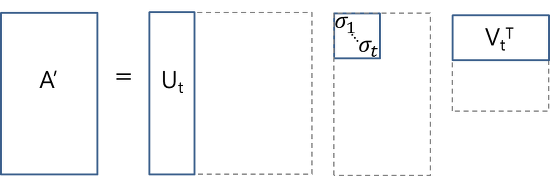
\includegraphics[width=\columnwidth]{svd.png}
  \end{multicols}

\end{frame}

\begin{frame}{Understand Latent Semantic Analysis}
  {\bf Topics are principle components of entire document collection}

  \begin{multicols}{2}
    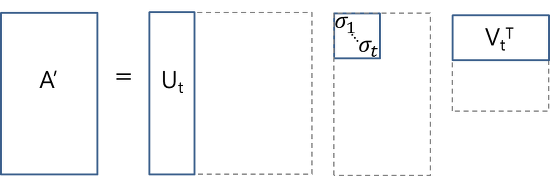
\includegraphics[width=\columnwidth]{svd.png}
    \columnbreak

    \begin{itemize}
      \item[{\bf U:}] document-topic matrix, topic contributes to document
      \item[{\bf S:}] singular values
      \item[{\bf V:}] word-topic matrix, topic contribute to words
    \end{itemize}
  \end{multicols}

  \begin{itemize}
  \item Overfit as consequence of topics strict mathematical definition
  \item Topics are better interpreted as mathematical than intuitive
  \item Cost of finding one topic is the same as finding all possible topics
  \end{itemize}
\end{frame}


\begin{frame}{Goals of generative models}
  {\bf A generative model}

  \begin{itemize}
  \item Assume/Generalize how data could have been generated
  \item Fit distributions that describe generalization
  \item Ask questions about the generalization in relation to data
  \item Ask questions about data in relation to the generalization
  \end{itemize}

  \vspace{1em}

  \begin{quote}
    Generative models are much easier to extend, because they abstract the model from it's linear algebra dependencies.

    \vspace{1em}

  Topic modeling generalizes how a document is generated by claiming that words come from topics, and documents have multiple topics.\footnote{this is not a language model} %Note that this ignores sentence structure, entities, authorship, or other things we may care about.

  \end{quote}

\end{frame}


\begin{frame}{Probabilistic Latent Semantic Analysis}
  {\bf Generative model for SVD}

  \[P(d,w):\rightarrow \texttt{document-term matrix}\]

    \begin{itemize}
    \item  $P(z|d)$ is the probability $z$ contributes to $d$
    \item  $P(w|z)$ is the probability $w$ contributes to $z$
    \end{itemize}

    \[P(D,W) = P(D)\sum_Z P(Z|D)P(W|Z)\]

    \[P(Z|D) \texttt{ and } P(W|Z) \sim \texttt{Multinomial}\]

\end{frame}

\begin{frame}{Understand Probabilistic Latent Semantic Analysis}
  {\bf A mapping to SVD}

  \begin{align*}
    P(D,W) &= P(D)\sum_Z P(Z|D)P(W|Z)\\
    &= \sum_Z \color{red}P(Z)\color{blue}P(D|Z)\color{green}P(W|Z)\\
    \texttt{remembering}&\\
    A &\approx\color{blue}U_t\color{red}S_t\color{green}V_t^T
  \end{align*}

  First generate the topic $Z$ then generate the word $W$

  \begin{itemize}
  \item P(D) is not parameterized, we don't observe new documents
  \item Tends to be softer than LSA, but still  overfits (grows with D)
  \item No longer use \texttt{tfidf} best replaced with \texttt{stopwords}\footnote{Usually top $.5-2\%$ of vocab}
  \end{itemize}

\end{frame}


\end{document}
